\documentclass[12pt]{article}
\usepackage{sbc-template}
\usepackage{graphicx,url}
\usepackage{float}
\usepackage[brazil]{babel}   
\usepackage[utf8]{inputenc}  
\usepackage{url}
\bibliographystyle{ieeetr}

     

\sloppy
	\title{ Simulação de Pool de Impressão Dístribuida Utilizando Socket \\ Exercício Computacional II - Sistemas Distribuídos}

\author{Rafael Gonçalves de Oliveira Viana\inst{1}  }


\address{Sistemas de Informação -- Universidade Federal do Mato Grosso do Sul
	(UFMS)\\
  	Caixa Postal 79400-000 -- Coxim -- MS -- Brazil
  \email{rafael.viana@aluno.ufms.br }
  \\\vspace*{10pt} \normalsize  \today{}
}

\begin{document} 

\maketitle

     
\begin{resumo} 	
  Este relatório introduz a arquitetura de uma Pool de Thread.
\end{resumo}

\section{Introdução}
 \cite{webservece}.
 
\section{Fundamentação Téorica} 

\subsection{Socket}
 Segundo \cite{socket}.\cite{conc}.
 
\subsubsection{Fluxo TCP}
 Da necessidade de dois computadores se comunicarem, surgiram diversos protocolos que permitissem tal troca de informação: o protocolo que vamos usar aqui é o TCP (Transmission Control Protocol).
\subsection{Problema de Concorrência}
 Da necessidade de dois computadores se comunicarem, surgiram diversos protocolos que permitissem tal troca de informação: o protocolo que vamos usar aqui é o TCP (Transmission Control Protocol) \cite{conc}.

\begin{figure}[H]
	\centering
	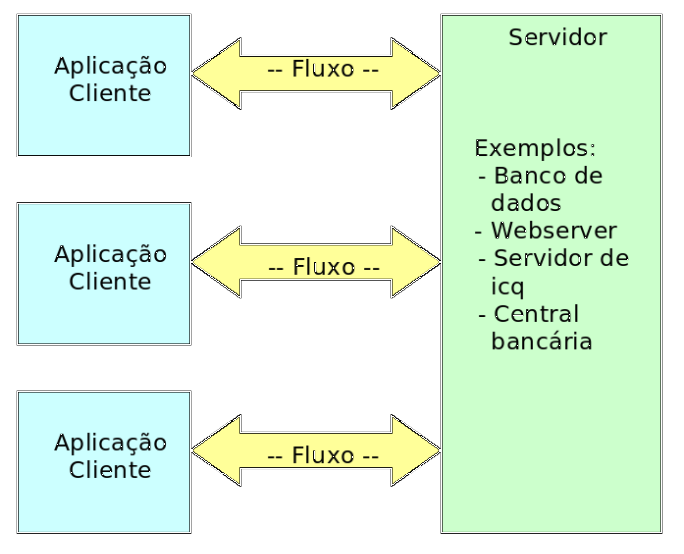
\includegraphics[scale=0.14]{imagens/fluxo.png}
	\caption{Conexão TCP.}
	\label{fluxotcp}
\end{figure} 
É possível conectar mais de um cliente ao mesmo servidor, como é o caso de diversos banco de dados, servidores Web, etc.

\section{Desenvolvimento}
\subsection{Clientes}

\subsection{Pool de Impressão}

\subsection{Impressoras}

\section{Conclusão}
Neste relatório foi apresentado a estrutura básica de um.


\bibliography{bibli}

\end{document}


